%\input{Preambulum}

\begin{figure}[t!]
\centering

\begin{subfigure}{\textwidth}
\caption{Graphs with pair constraints ($G_1$--$G_{31}$, Figure~\ref{Fig1})}
\label{Fig5a}

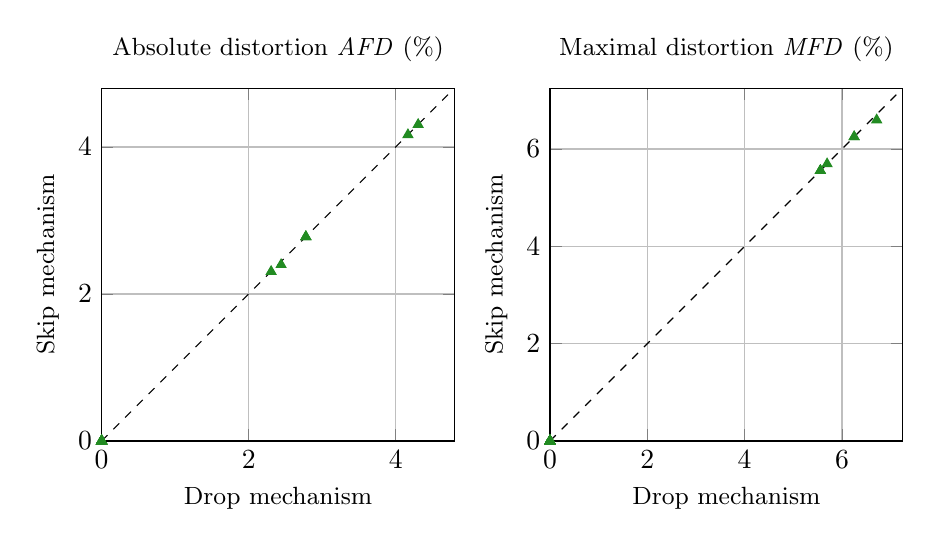
\begin{tikzpicture}
\begin{axis}[
name = axis1,
title = {Absolute distortion $\mathit{AFD}$ (\%)},
title style = {font=\small},
xlabel = Drop mechanism,
x label style = {font=\small},
ylabel = Skip mechanism,
y label style = {font=\small},
width = 0.5\textwidth,
height = 0.5\textwidth,
nodes near coords,
xmajorgrids = true,
ymajorgrids = true,
xmin = 0,
xmax = 4.8,
ymin = 0,
ymax = 4.8,
]
\addplot [scatter,red,only marks,mark size=1.5pt,point meta=explicit symbolic] coordinates {
};
\addplot [scatter,blue,only marks,mark=x,mark size=2.5pt,thick,point meta=explicit symbolic] coordinates {
};
\addplot [scatter,ForestGreen,only marks,mark=triangle*,mark size=2pt,point meta=explicit symbolic] coordinates {
(0,0)
(2.44107744107744,2.3989898989899)
(0,0)
(4.30555555555557,4.30555555555556)
(2.30555555555551,2.30555555555556)
(0,0)
(0,0)
(4.16666666666667,4.16666666666667)
(0,0)
(0,0)
(2.7777777777778,2.77777777777778)
(0,0)
(2.7777777777778,2.77777777777778)
(0,0)
(0,0)
(0,0)
(0,0)
(0,0)
(0,0)
(2.7777777777778,2.77777777777778)
(0,0)
(0,0)
(0,0)
(0,0)
(0,0)
(0,0)
(0,0)
};
% Zero line
\draw [black,dashed] (rel axis cs:0,0) -- (rel axis cs:1,1);
\end{axis}

\begin{axis}[
at = {(axis1.south east)},
xshift = 0.1\textwidth,
title = {Maximal distortion $\mathit{MFD}$ (\%)},
title style = {font=\small},
xlabel = Drop mechanism,
x label style = {font=\small},
ylabel = Skip mechanism,
y label style = {font=\small},
width = 0.5\textwidth,
height = 0.5\textwidth,
nodes near coords,
xmajorgrids = true,
ymajorgrids = true,
xmin = 0,
xmax = 7.25,
ymin = 0,
ymax = 7.25,
]
\addplot [scatter,red,only marks,mark size=1.5pt,point meta=explicit symbolic] coordinates {
};
\addplot [scatter,blue,only marks,mark=x,mark size=2.5pt,thick,point meta=explicit symbolic] coordinates {
};
\addplot [scatter,ForestGreen,only marks,mark=triangle*,mark size=2pt,point meta=explicit symbolic] coordinates {
(0,0)
(6.71296296296298,6.59722222222223)
(0,0)
(6.25000000000006,6.25)
(5.69444444444444,5.69444444444444)
(0,0)
(0,0)
(6.25,6.25)
(0,0)
(0,0)
(5.55555555555556,5.55555555555555)
(0,0)
(5.55555555555556,5.55555555555555)
(0,0)
(0,0)
(0,0)
(0,0)
(0,0)
(0,0)
(5.55555555555556,5.55555555555555)
(0,0)
(0,0)
(0,0)
(0,0)
(0,0)
(0,0)
(0,0)
};
% Zero line
\draw [black,dashed] (rel axis cs:0,0) -- (rel axis cs:1,1);
\end{axis}
\end{tikzpicture}
\end{subfigure}

\vspace{0.25cm}
\begin{subfigure}{\textwidth}
\caption{Graphs without pair constraints ($H_1$--$H_{31}$, Figure~\ref{Fig2})}
\label{Fig5b}

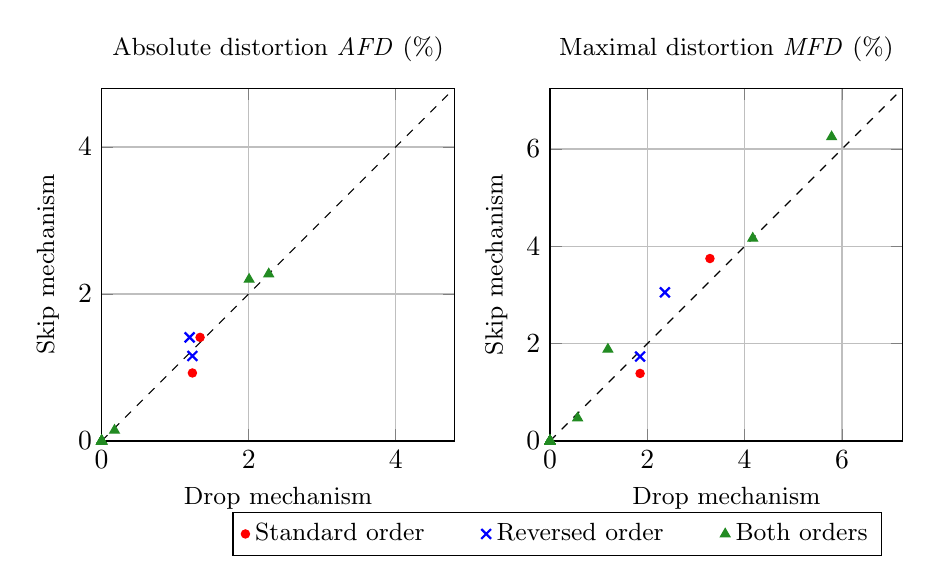
\begin{tikzpicture}
\begin{axis}[
name = axis1,
title = {Absolute distortion $\mathit{AFD}$ (\%)},
title style = {font=\small},
xlabel = Drop mechanism,
x label style = {font=\small},
ylabel = Skip mechanism,
y label style = {font=\small},
width = 0.5\textwidth,
height = 0.5\textwidth,
nodes near coords,
xmajorgrids = true,
ymajorgrids = true,
xmin = 0,
xmax = 4.8,
ymin = 0,
ymax = 4.8,
]
\addplot [scatter,red,only marks,mark size=1.5pt,point meta=explicit symbolic] coordinates {
(1.33903133903132,1.41025641025641)
(1.23456790123459,0.925925925925925)
};
\addplot [scatter,blue,only marks,mark=x,mark size=2.5pt,thick,point meta=explicit symbolic] coordinates {
(1.19658119658119,1.41025641025641)
(1.23456790123457,1.15740740740741)
};
\addplot [scatter,ForestGreen,only marks,mark=triangle*,mark size=2pt,point meta=explicit symbolic] coordinates {
(0,0)
(0,0)
(0.680272108843538,10.7709750566894)
(0.174825174825178,0.145687645687649)
(0,0)
(0,0)
(0,0)
(2.00617283950617,2.19907407407407)
(2.2727272727273,2.27272727272727)
(0,0)
(0,0)
(0,0)
(0,0)
(0,0)
(0,0)
(0,0)
(0,0)
(0,0)
};
% Zero line
\draw [black,dashed] (rel axis cs:0,0) -- (rel axis cs:1,1);
\end{axis}

\begin{axis}[
at = {(axis1.south east)},
xshift = 0.1\textwidth,
title = {Maximal distortion $\mathit{MFD}$ (\%)},
title style = {font=\small},
xlabel = Drop mechanism,
x label style = {font=\small},
ylabel = Skip mechanism,
y label style = {font=\small},
width = 0.5\textwidth,
height = 0.5\textwidth,
nodes near coords,
xmajorgrids = true,
ymajorgrids = true,
xmin = 0,
xmax = 7.25,
ymin = 0,
ymax = 7.25,
legend style = {font=\small,at={(-0.9,-0.2)},anchor=north west,legend columns=3},
legend entries = {Standard order$\qquad$,Reversed order$\qquad$,Both orders}
]
\addplot [scatter,red,only marks,mark size=1.5pt,point meta=explicit symbolic] coordinates {
(3.28703703703703,3.75)
(1.85185185185196,1.38888888888889)
};
\addplot [scatter,blue,only marks,mark=x,mark size=2.5pt,thick,point meta=explicit symbolic] coordinates {
(2.36111111111115,3.05555555555556)
(1.85185185185187,1.73611111111111)
};
\addplot [scatter,ForestGreen,only marks,mark=triangle*,mark size=2pt,point meta=explicit symbolic] coordinates {
(0,0)
(0,0)
(1.19047619047619,1.88492063492063)
(0.568181818181826,0.473484848484848)
(0,0)
(0,0)
(0,0)
(5.78703703703703,6.25)
(4.1666666666668,4.16666666666667)
(0,0)
(0,0)
(0,0)
(0,0)
(0,0)
(0,0)
(0,0)
(0,0)
(0,0)
};
% Zero line
\draw [black,dashed] (rel axis cs:0,0) -- (rel axis cs:1,1);
\end{axis}
\end{tikzpicture}
\end{subfigure}

\caption{Fairness distortions of the draw mechanisms \\ for balanced bipartite graphs with eight nodes ($n=4$)}
\label{Fig5}
\end{figure}

%\end{document}
